\chapter{Titel derde hoofdstuk}

Vul aan.


\lipsum[20-24]

\section{Sectie titel}

Vul aan.

\lipsum[32-34]
\section{Sectie titel2}

\lipsum[6-8]

Voorbeeld figuur.

\begin{figure}
	\centering
	\begin{subfigure}{\textwidth}
		\centering
		\centerline{
			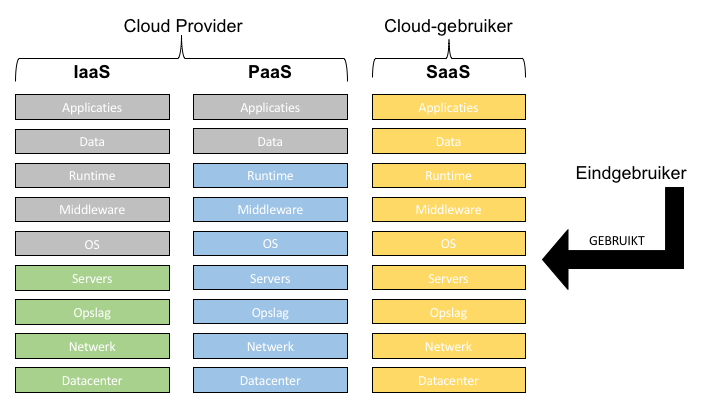
\includegraphics[scale=0.47]{cloud_rollen}
		}
	\end{subfigure}
	\caption{Cloudstakeholders met de bijhorende cloudvorm.}
	\label{fig:cloud_rollen}
\end{figure}

\subsection*{Subtitel}
\addcontentsline{toc}{subsection}{Subtitel}  
Vul aan
\subsection{Functie is\_isbn}

Voorbeeld listing.

\begin{code}
\inputminted{python}{isbn.py}
\caption{Functie is\_isbn}
\end{code}